\section{Initial Experiments}

With our theoretical understanding of the Wi-Fi standard and its capabilities, we move on to looking at the Wi-Fi landscape in real-world.
We achieve this by designing small independent experiments where we record the Wi-Fi probe requests within controlled conditions along with the knowledge of the ambient population of the field of measurement. 
We then look at the collected probe requests, examine them in detail to look at their properties, aggregate them to footfall counts and compare them with the real-world counts to get a overall idea of how well they translate into real counts.
The aim of these experiments to know more about the probe requests data and pick out the uncertainties and opportunities present in them.
The objectives here are,

\begin{enumerate}
  \setlength{\itemindent}{2em}
  \itemsep-0.25em
   \item Design a simple method to collect probe requests.
  \item Select locations with different levels of complexity.
  \item Collect real-world data through manual counting.
  \item Analyse the probe requests to extract useful information.
\end{enumerate}

\subsection{Experiment Design}

The first step was to design a simple method to collect Wi-Fi probe requests.
We accomplish by utilising the application - \textit{tshark} \cite{wireshark2} on a regular laptop.
First we put the Wi-Fi module of the laptop in `Monitor mode' where it behaves as a wireless access point.
Then we run tshark to collect the data in CSV format using the following command under a shell.

\begin{minted}{bash}
#! /bin/bash
tshark \
  -I -i en0 \
  -T fields \
  -E separator=, \
  -E quote=d \
    -e frame.time \
    -e frame.len \
    -e wlan_radio.signal_dbm \
    -e wlan_radio.duration \
    -e wlan.sa_resolved \
    -e wlan.seq \
    -e wlan.tag.length \
    -e wlan.ssid \
  type mgt subtype probe-req and broadcast
\end{minted}

The fields marked with \textit{-e} correspond to time stamp when the packet was received, total length of the packet, reported signal strength, duration for which the packet was transmitted, the MAC address of the source device, sequence number of the packet assigned by the source device, length of the tags attached to the packet and the network for which the probe request is being sent for.
The manufacturer information is extracted from the \textit{wlan.sa\_resolved} field into a separate column and the original field is hashed using the SHA256 algorithm implemented in R.
In addition to this, the pedestrians next to the sensor were counted manually by the surveyor.

\subsection{Living room}

\begin{marginfigure}
  \forcerectofloat
  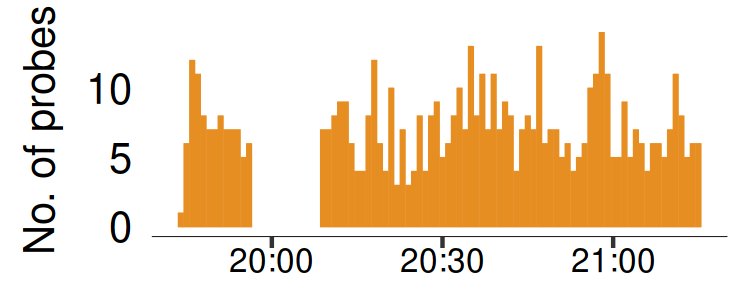
\includegraphics{images/home-total-count.png}
  \caption{Number of probe requests collected every minute on 15 October 2017}
  \label{figure:collection:home:total}
\end{marginfigure}

The first set of experiment was conducted with the laptop in the researcher's living room. 
The room was known to have 2 phones and an Android TV device and the whole house had an occupancy of 3.
Probe requests were collected on 15 Nov 2015 from 19:44 to 21:15 with a gap of 15 minutes in between.
We collected around 3000 probe requests at the rate of 38 requests per minute.
The total number of probe requests collected every minute is shown in Figure \ref{figure:collection:home:total}.

The first thing we looked to convert this to footfall is the mac address along with OUIs.
Initial thoughts on this.
We found that it is not enough.
Strong evidence that mac address randomisation is affecting the numbers.

Other information that can help here - Signal strength, tags, SSID, length, sequence numbers and duration.
Signal strength shows promise!
Length seems useful as it give uniqueness!
Duration and length are directly related and gives no extra information.
SSID and tags have very low or varied data they have no use.
Sequence numbers are interesting and shows most promise.
We need to see the variation and usefulness of length, so need more data.

\subsection{University Hall}
This was conducted to examine the previous results in a larger set of data in a real world setting.
Conducted in one of the main corridors - Southern cloisters of UCL with lot of pedestrian traffic.
There were also seating areas across the corridor where students work with their computers.
The area is also used heavily for lunch for large contingent of visitors.
Collected around 14750 probe requests collected and 652 users were counted walking around the sensors manually.

Major conclusion is that confirmation that Signal strength is still useful.
Length information is not that useful in certain standardised manufacturers.

\subsection{Oxford Street}

Aim is to validate the filtering and clustering methodology against the scale and complexity of data collected in an open public area such as a retail high street.
We also aimed to find the algorithm which was best suited for the classification of signal strengths as 'low' and 'high' in order to filter out the background noise.
The data was collected at Oxford Street, London on 20 December 2017 from 12:30 to 13:00 hrs, Wi-Fi probe requests were collected using the sensor described in Section and pedestrian footfall was manually recorded using the Android app - Clicker bala2018clicker.
Being located at one of the busiest retail locations in the United Kingdom, the Wi-Fi sensor captured approximately 60,000 probe requests during the half hour period; 3,722 people were manually recorded walking on the pavement during that time.
The surveyor positioned himself at the front of a store while carrying the sensor in a backpack and counted people walking by the store on the pavement (3m wide approximately) using a mobile phone.
The sensor was kept as close to the store window as possible, and the manual count was done as a cordon count in front of the store.

The analysis and use of this dataset is 

\subsection{Summary and Discussion}
